
\section{Research Objective 5: Case Studies and Benchmarks}
\begin{frame}
    \Large{\centerline{\textbf{Research Objective 5}}}
    \vspace{6pt}
    \large{\centerline{\textbf{Case Studies and Benchmarks}}}
\end{frame}

\subsection{Aralia Fault Tree Data Set}
\begin{frame}[t]
\frametitle{Overview: Aralia Dataset}
\begin{itemize}
  \item \textbf{Dataset Composition:} The Aralia collection consists of 43 distinct fault trees, each with varying numbers of basic events (BEs), gate types (AND, OR, K/N, XOR), and minimal cut-set counts.  
  \item \textbf{Diverse Problem Sizes:} Small trees (e.g.\ 25--32 BEs) through large models with over 1{,}500 BEs.  
  \item \textbf{Wide Probability Range:} Top-event probabilities spanning from rare events near \(10^{-13}\) to fairly likely failures with probability above 0.7.  
  \item \textbf{Model Variability:} Some trees are primarily AND/OR, others incorporate more advanced gates (K/N, XOR, NOT), providing thorough coverage of typical (and atypical) fault tree logic structures.
\end{itemize}
\end{frame}

\begin{frame}[allowframebreaks]
    \input{4_casestudy/3_table_aralia_ft_dataset}
\end{frame}

\subsection{Benchmarking Procedure}
\begin{frame}[t]
\frametitle{Benchmarking Setup: Hardware and Environment}
\begin{itemize}
  \item \textbf{Target Hardware:}
    \begin{itemize}
      \item GPU: NVIDIA\textsuperscript{\textregistered} GeForce GTX 1660 SUPER (6\,GB GDDR6, 1{,}408 CUDA cores).
      \item CPU: Intel\textsuperscript{\textregistered} Core\textsuperscript{TM} i7-10700 (2.90\,GHz, turbo-boost, hyperthreading).
    \end{itemize}
  \item \textbf{Software Stack:}
    \begin{itemize}
      \item SYCL-based (AdaptiveCpp/HipSYCL), with LLVM-IR JIT for kernel compilation.
      \item Compiler optimization at \texttt{-O3} for efficient code generation.
      \item Repeated runs (5+) to mitigate transient variations.
    \end{itemize}
  \item \textbf{Measured Time:} Includes entire wall-clock duration, from host-device transfers and JIT compilation to final result collection.
\end{itemize}
\end{frame}

\subsection{Accuracy Benchmarks}
\begin{frame}
    \begin{figure}[h]
    \centering
    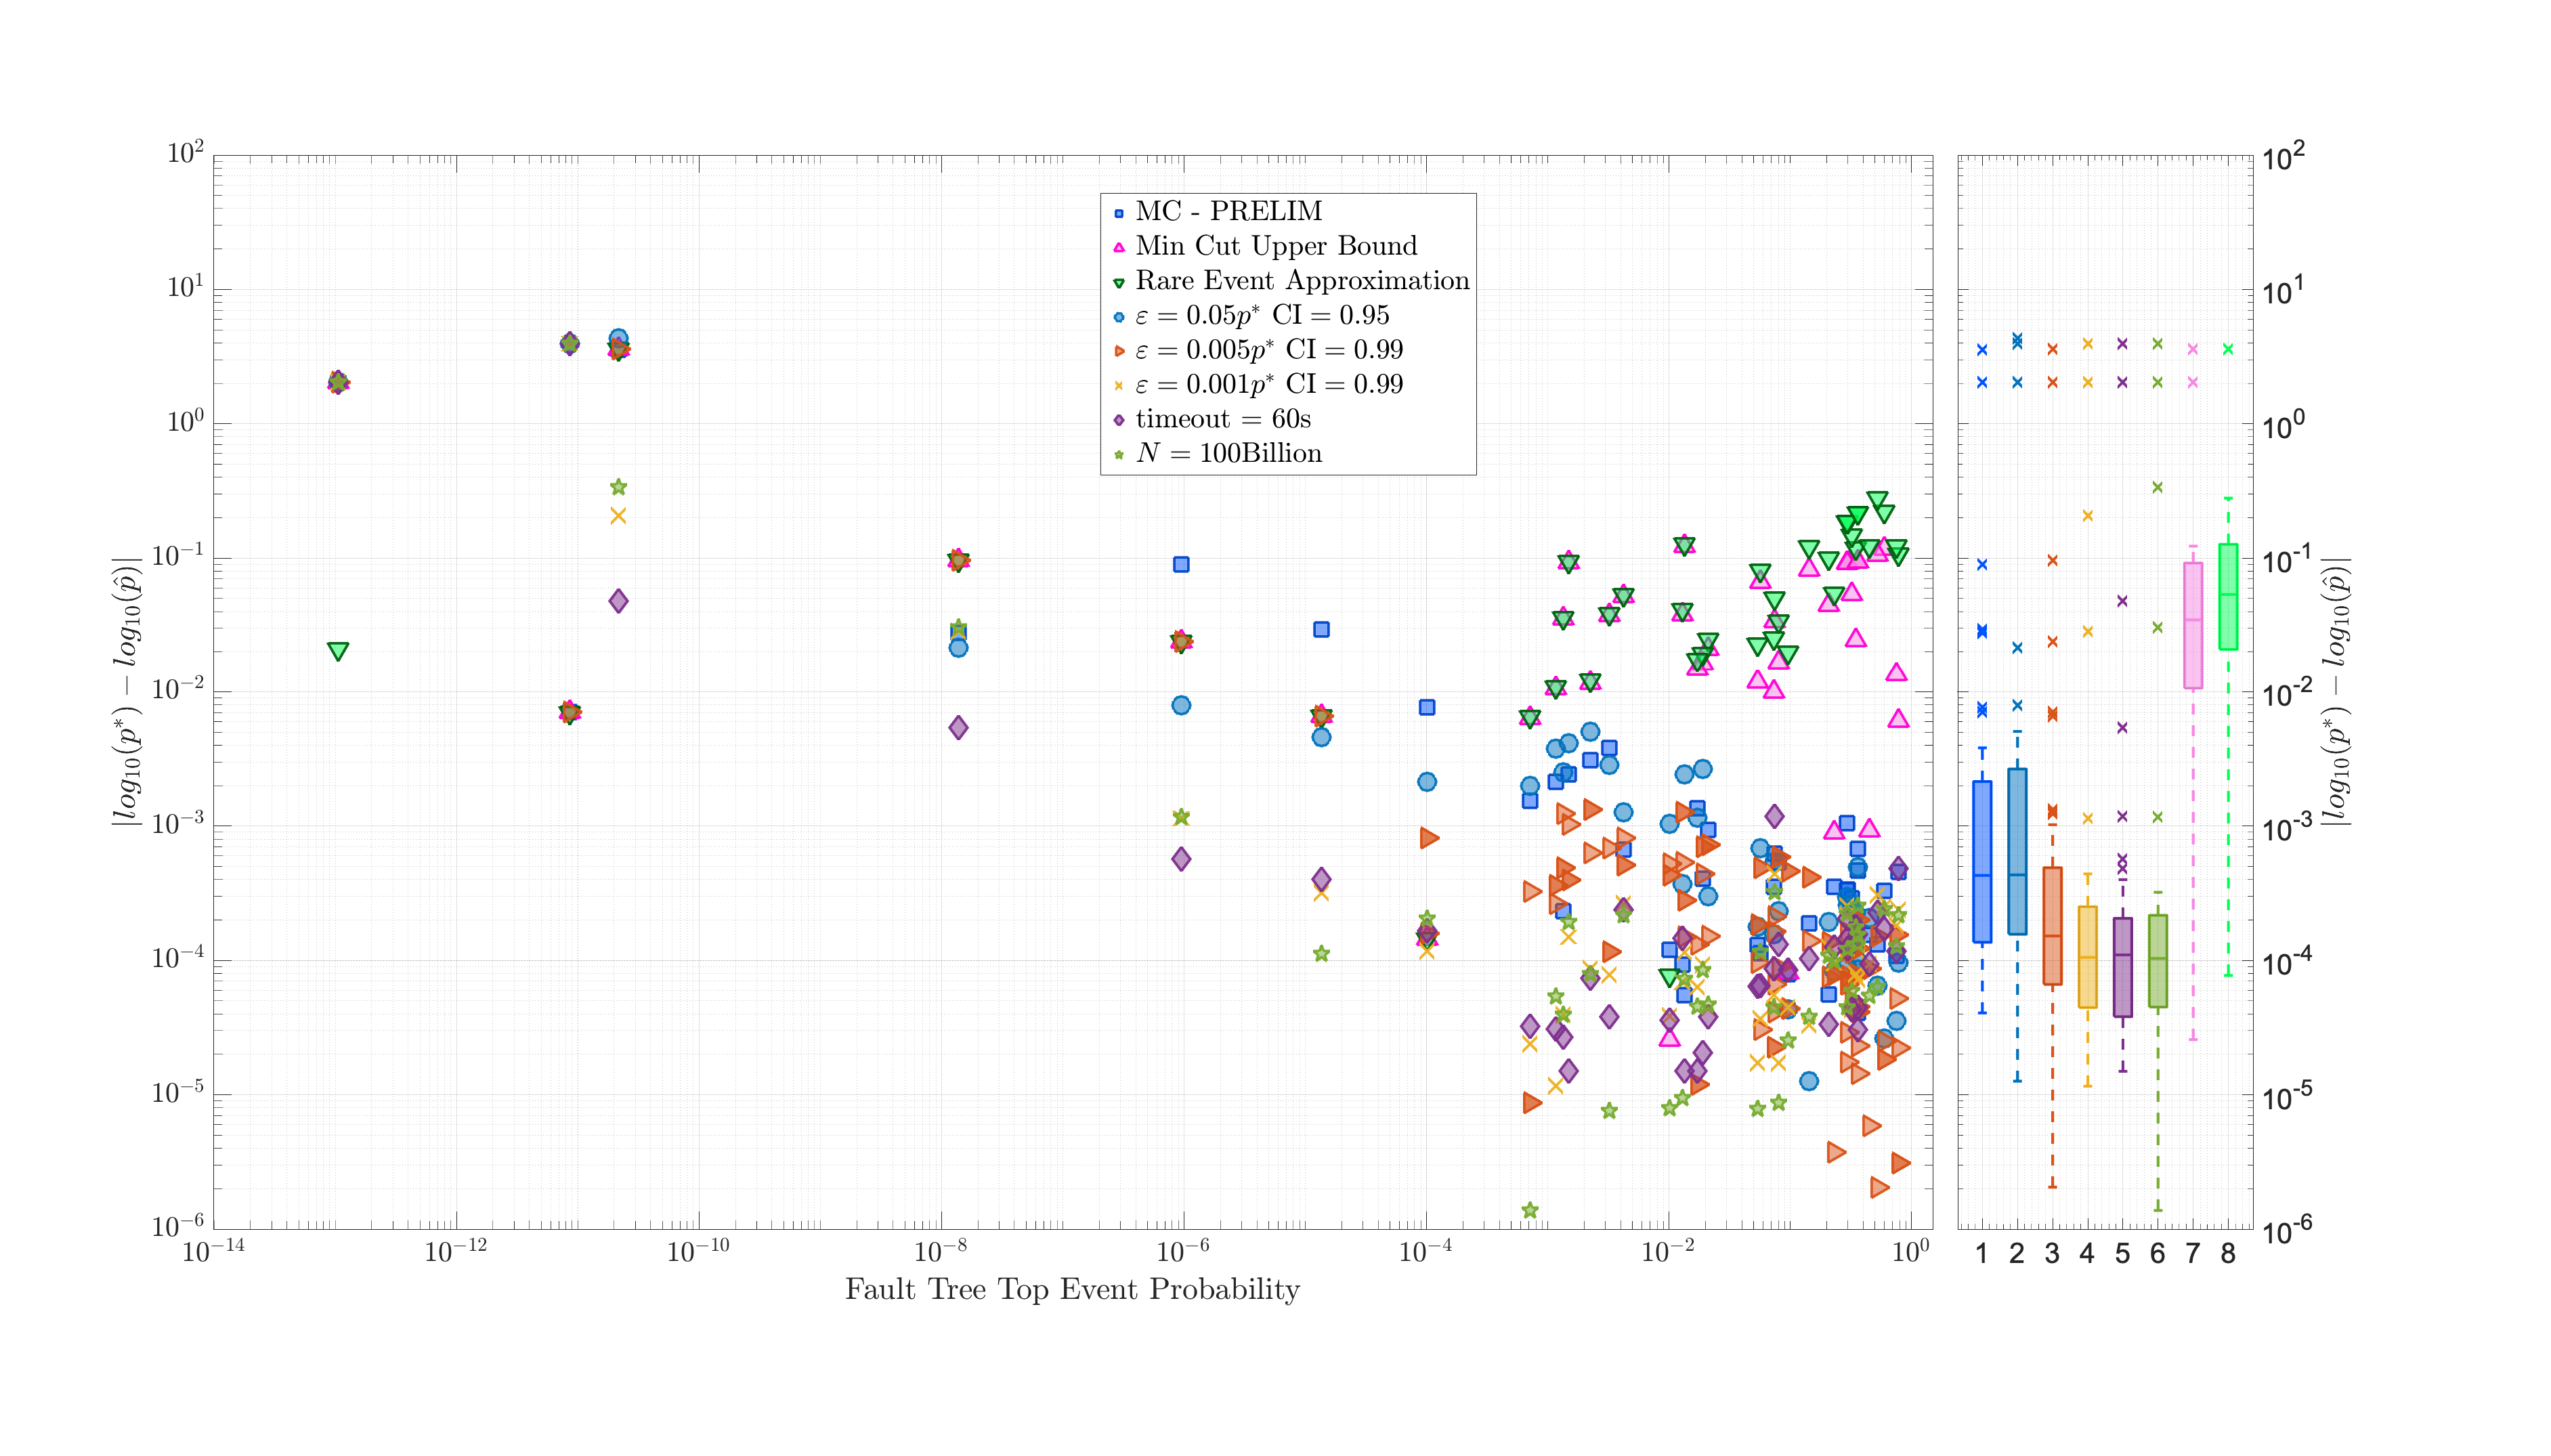
\includegraphics[height=1.1\textheight]{4_casestudy/abs_err.eps}
    \label{fig:mae_vs_logp}
\end{figure}
\end{frame}

\subsection{Accuracy vs. Time to Convergence}
\begin{frame}
\begin{figure}[p]
    \centering
    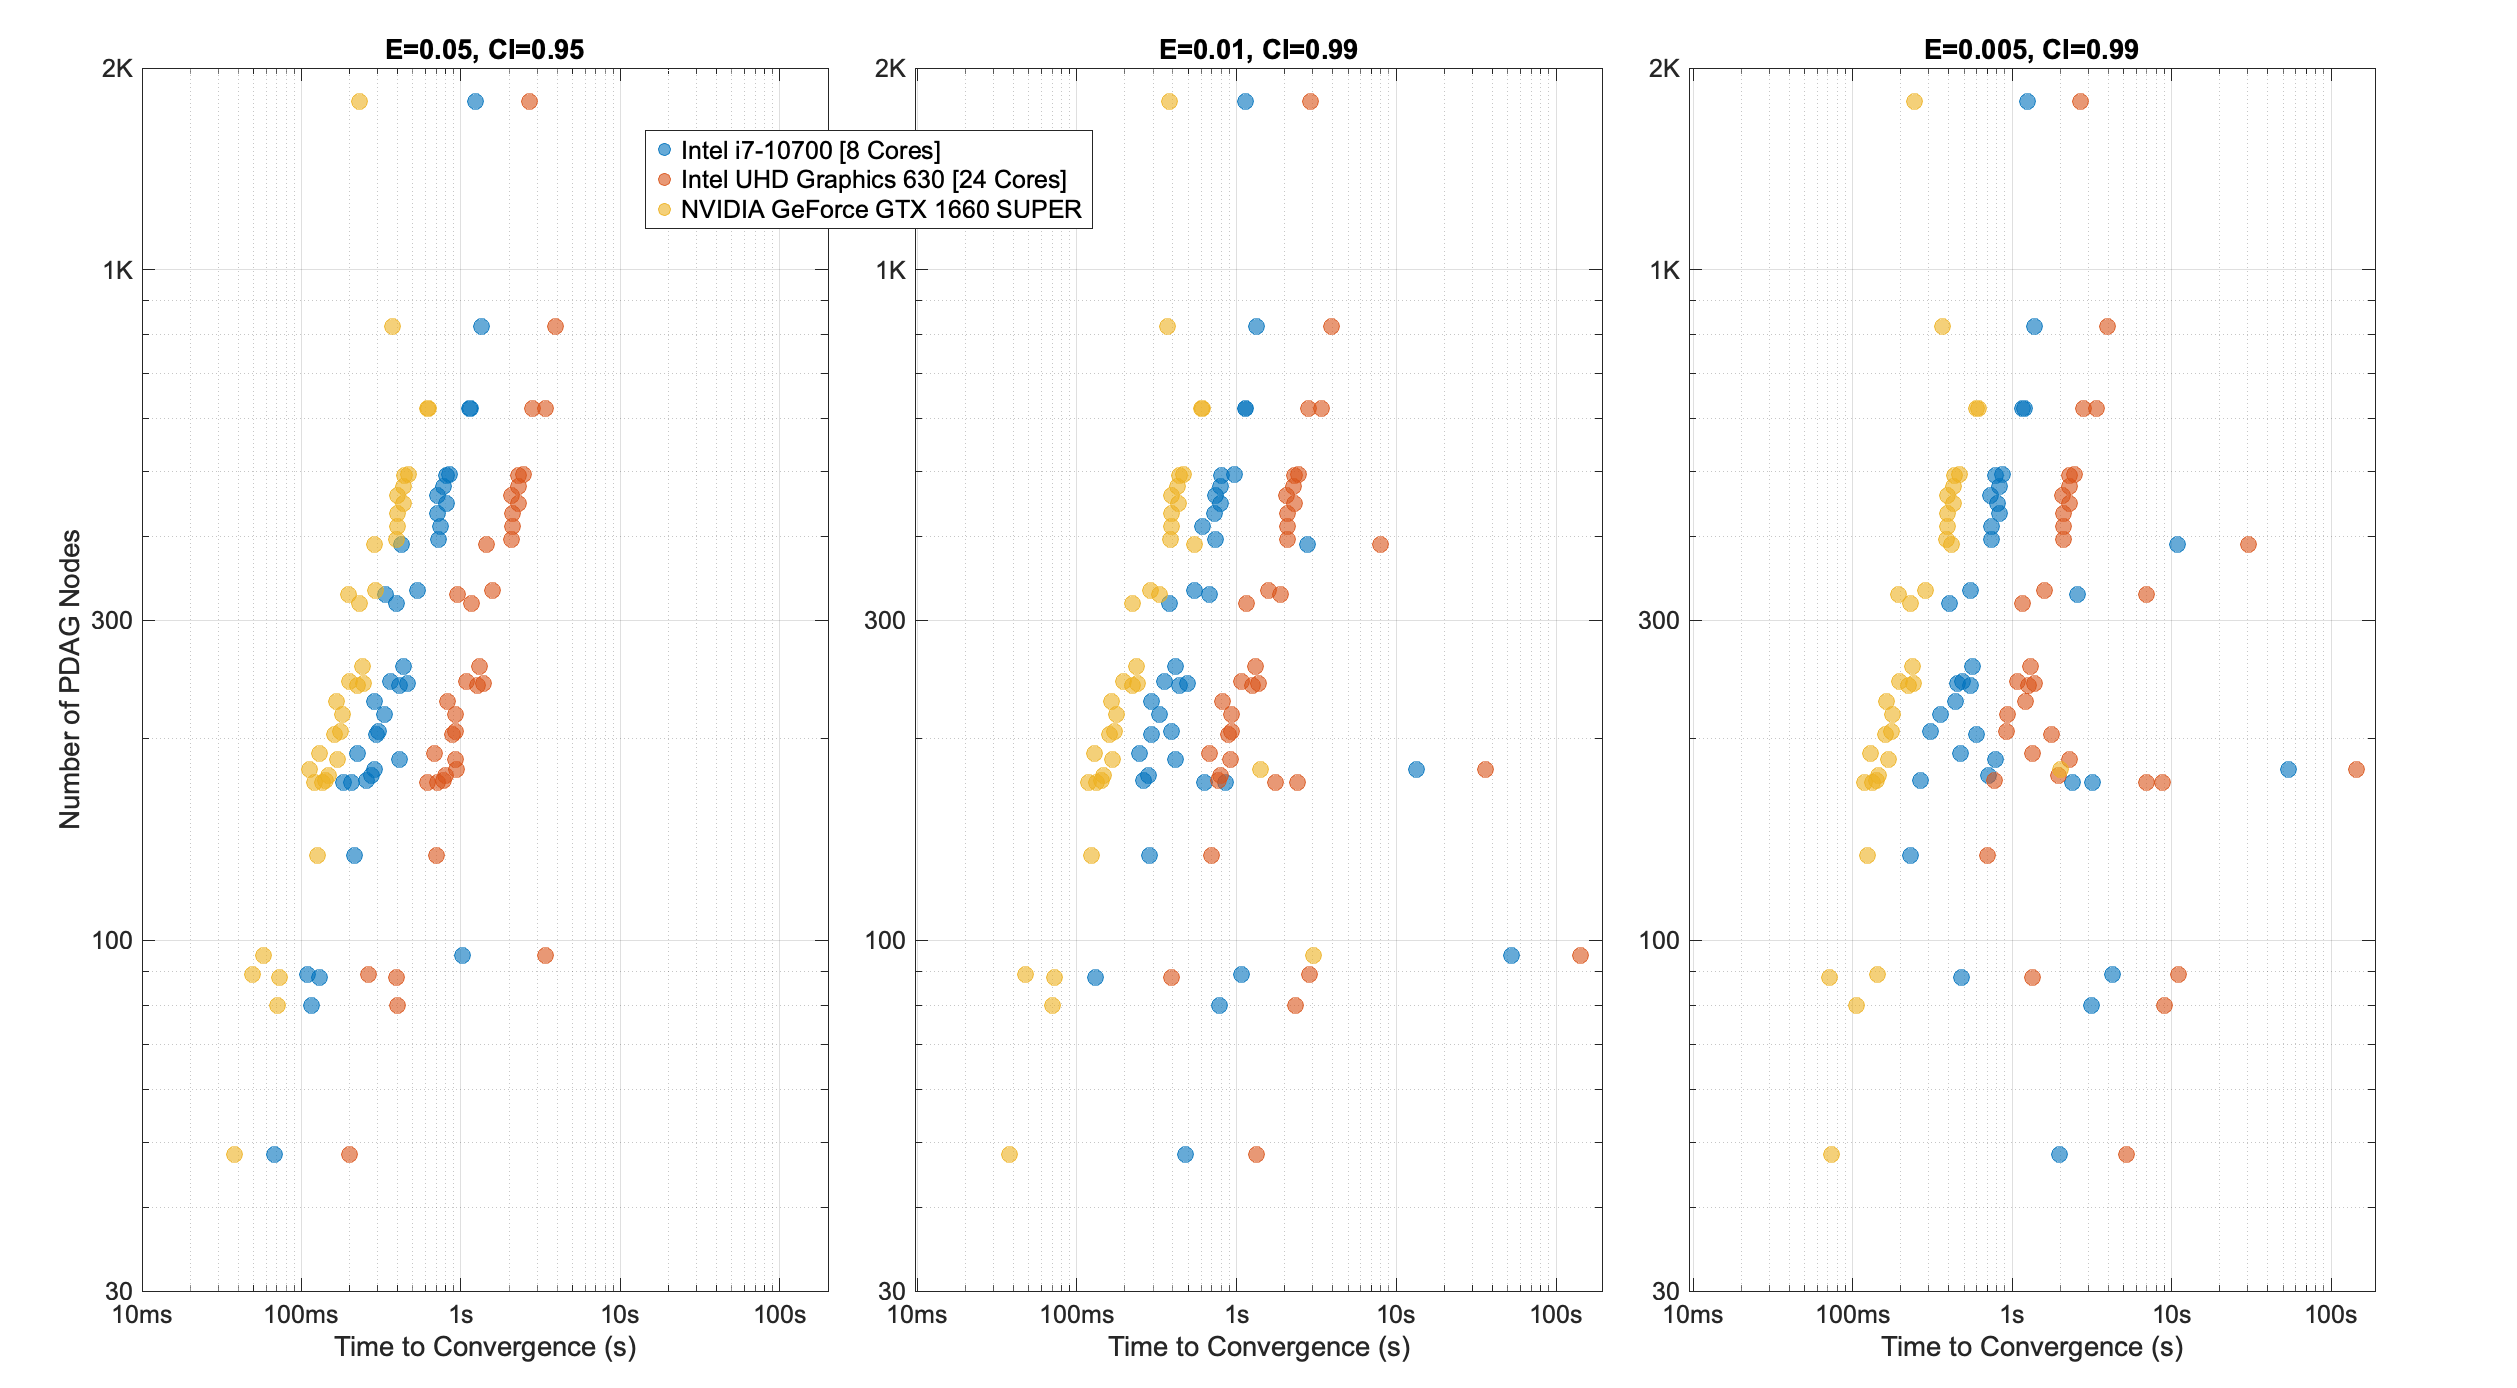
\includegraphics[height=1\textheight]{4_casestudy/throughput/slides_nodes_vs_convergence.eps}
    \caption{Time to convergence for different accuracy targets.}
    \label{fig:nodes_vs_convergence}
\end{figure}
\end{frame}

\subsection{Convergence Runs}
\begin{frame}
\begin{figure}[p]
    \centering
    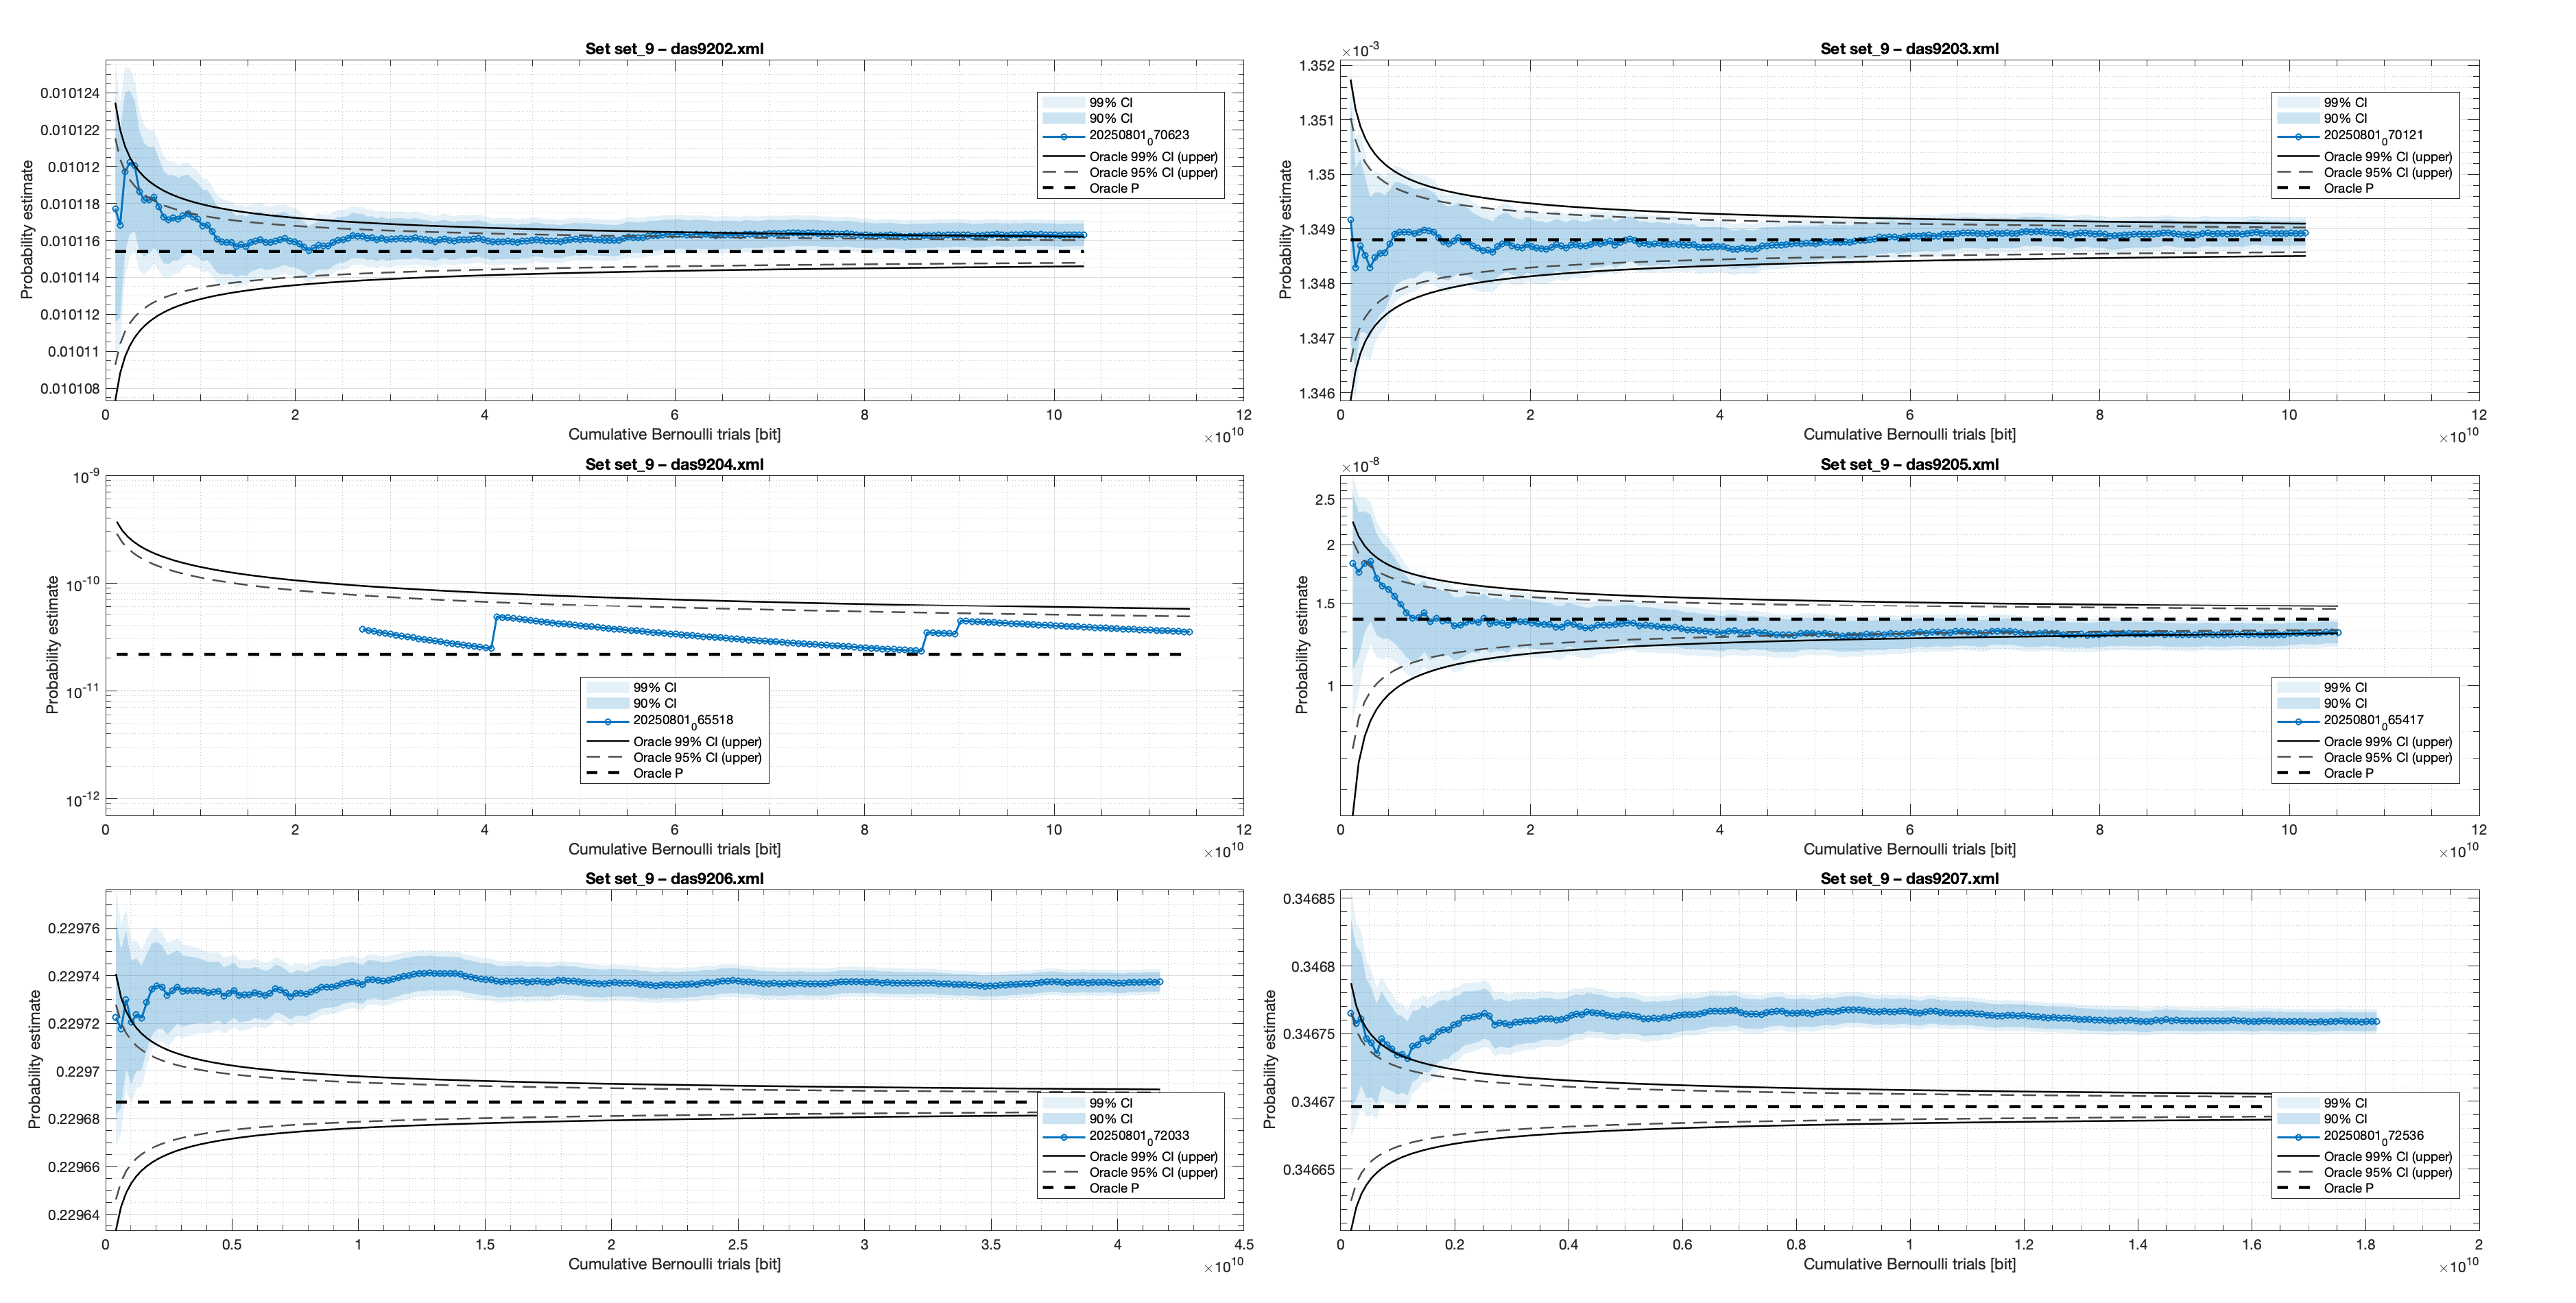
\includegraphics[height=1\textheight]{4_casestudy/conv_raw.eps}
    \label{fig:convergence_run_01}
\end{figure}
\end{frame}

\subsection{Convergence Runs, Comparison with MCUB, REA}
\begin{frame}
\begin{figure}[p]
    \centering
    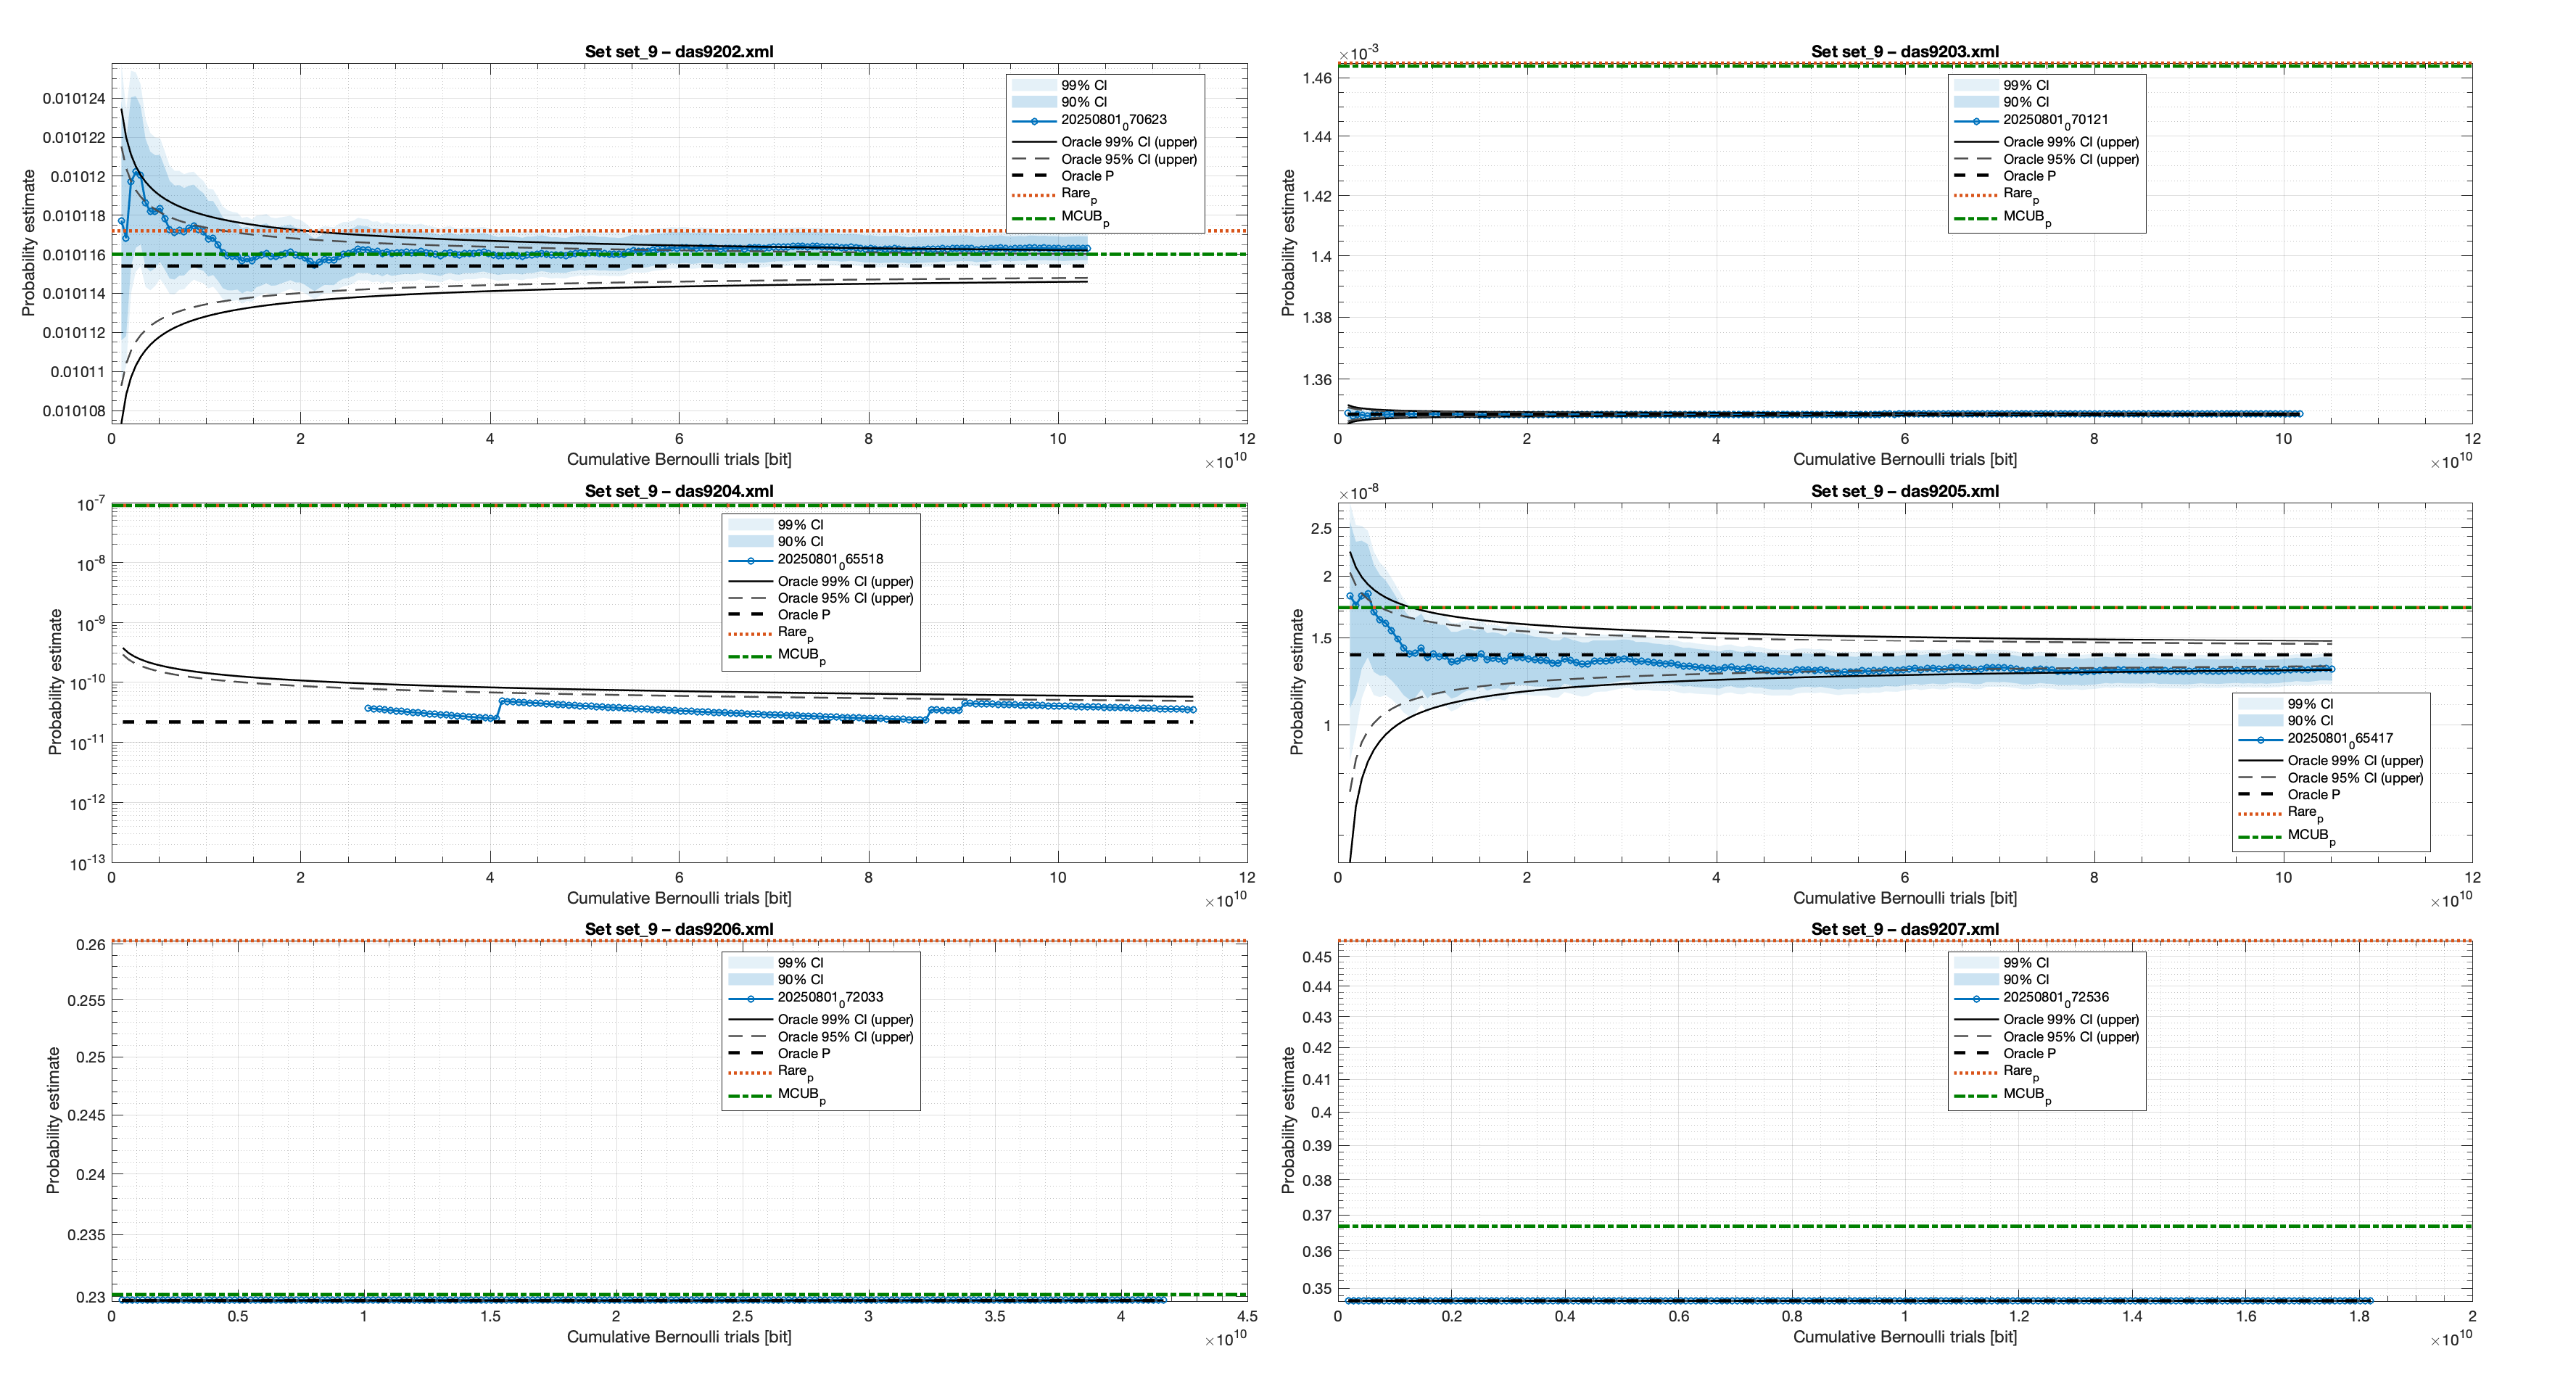
\includegraphics[height=1\textheight]{4_casestudy/conv_figeps.eps}
    \label{fig:convergence_run_01}
\end{figure}
\end{frame}

\subsection{Convergence Run -- Rare Event, Comparison with MCUB}
\begin{frame}
\begin{figure}[p]
    \centering
    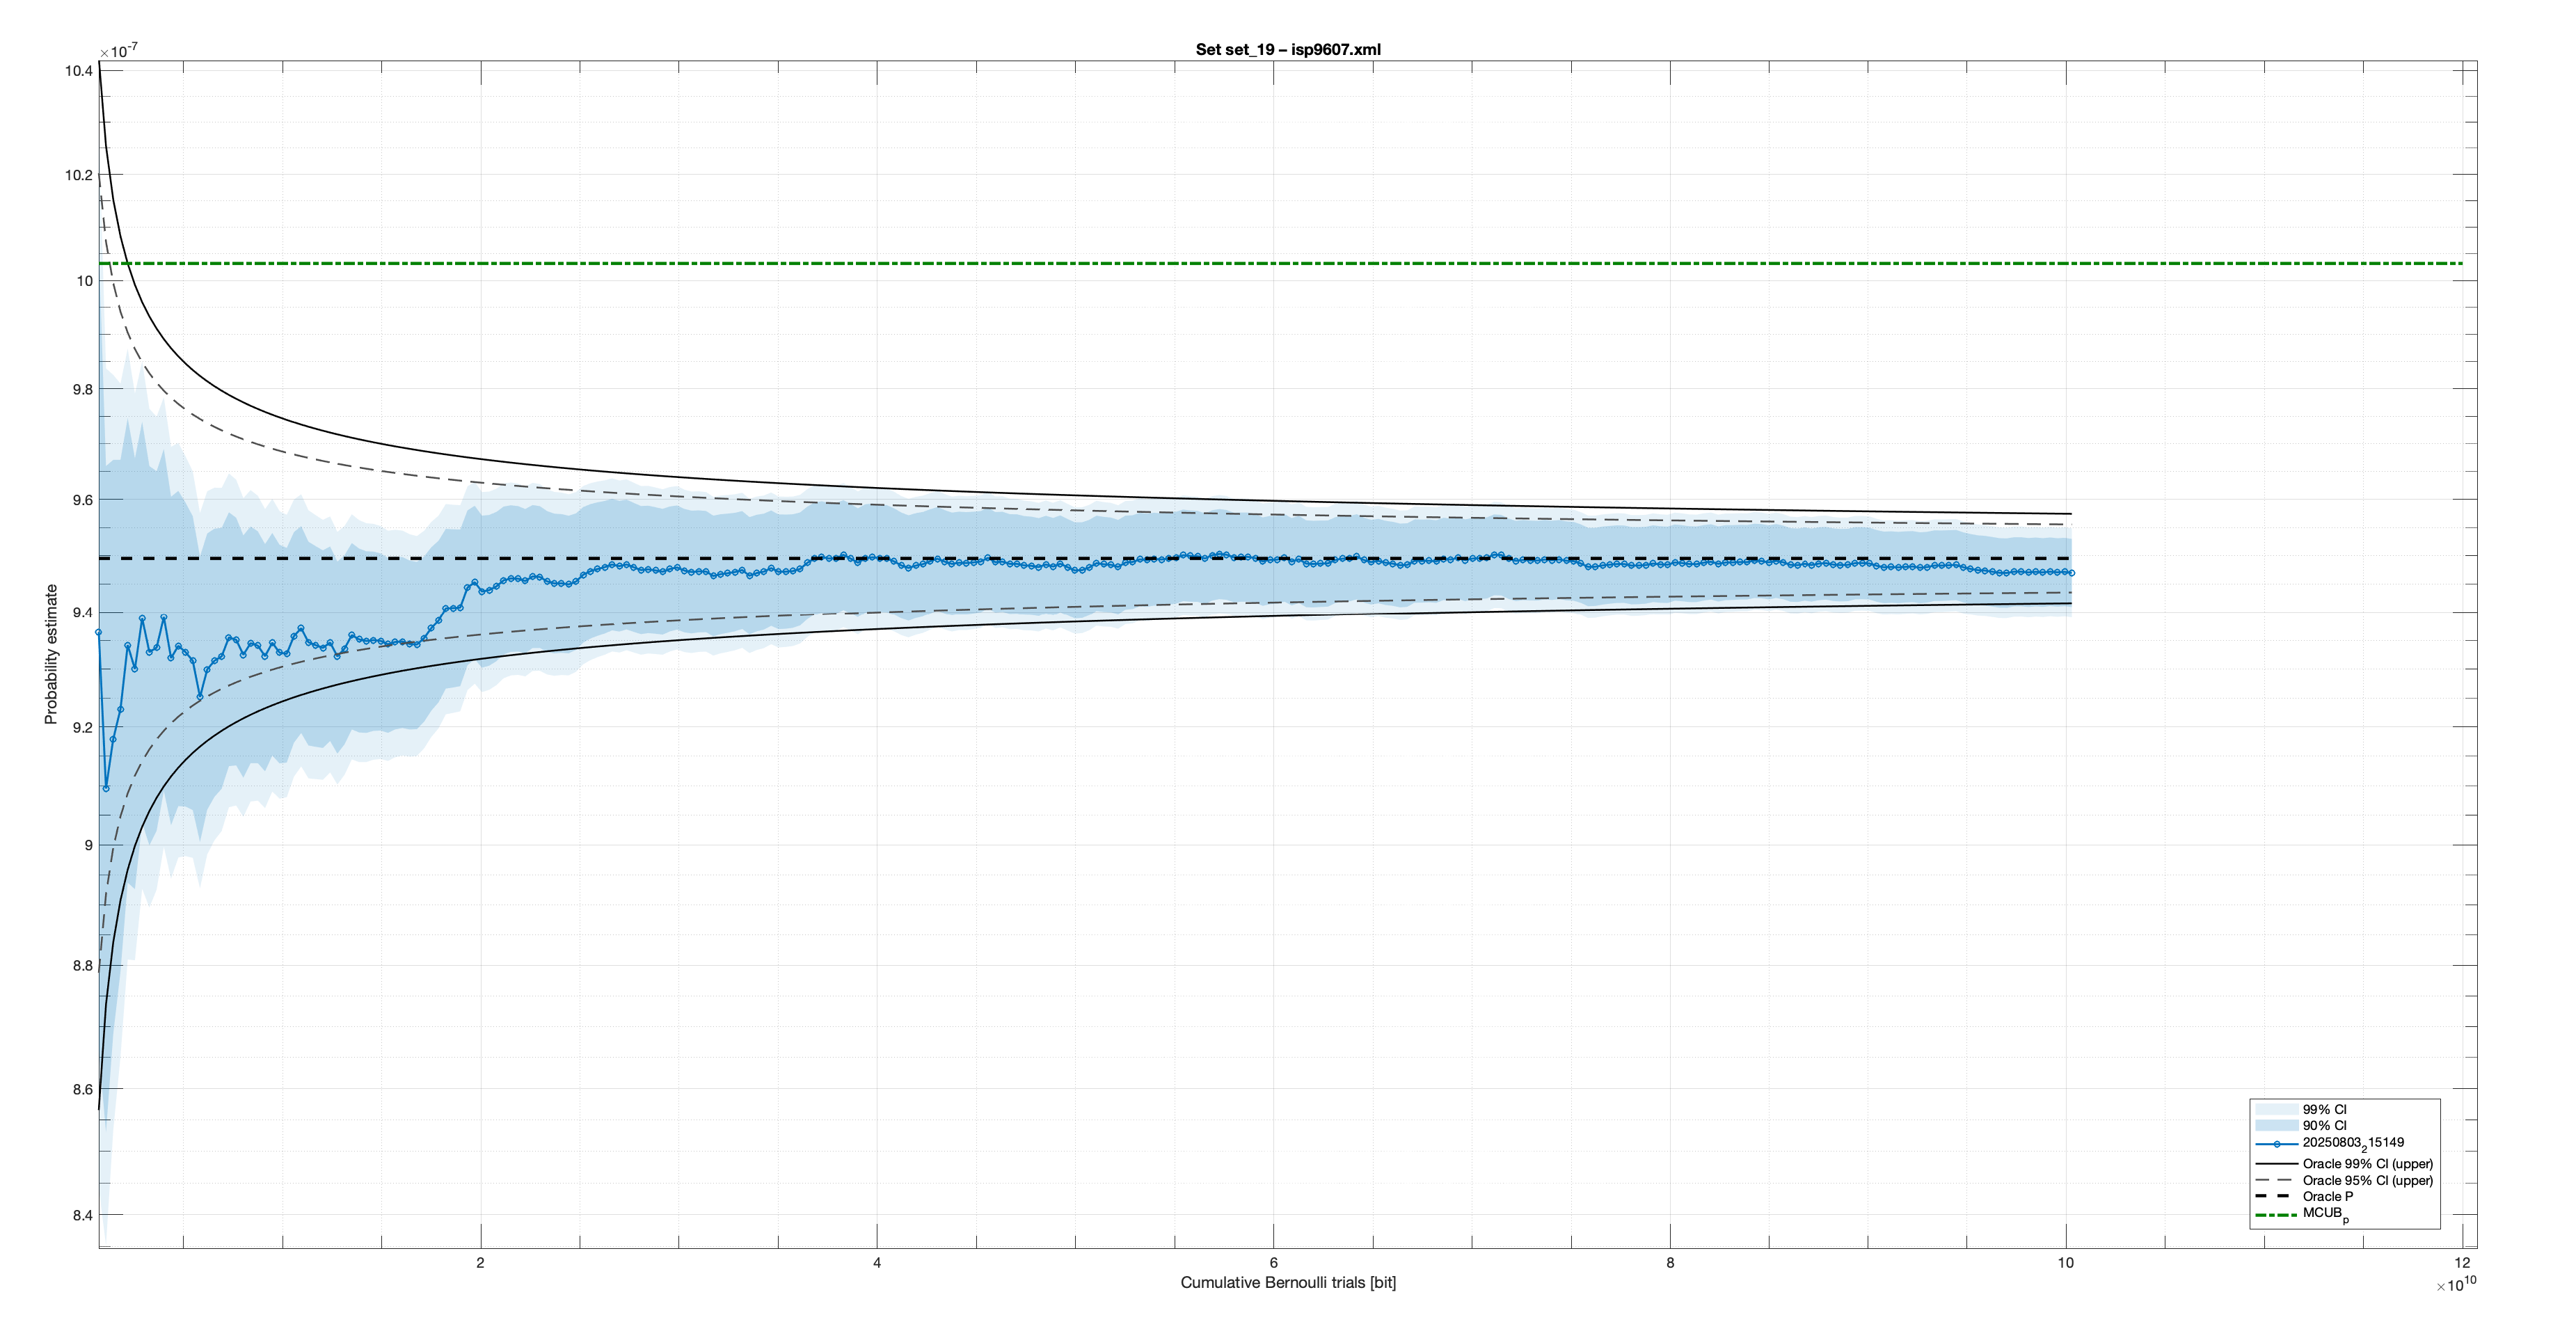
\includegraphics[height=0.9\textheight]{4_casestudy/conv_ips9607.eps}
    \label{fig:convergence_run_01}
\end{figure}
\end{frame}

\subsection{Convergence Free Run}
\begin{frame}
    \begin{figure}[h]
    \centering
    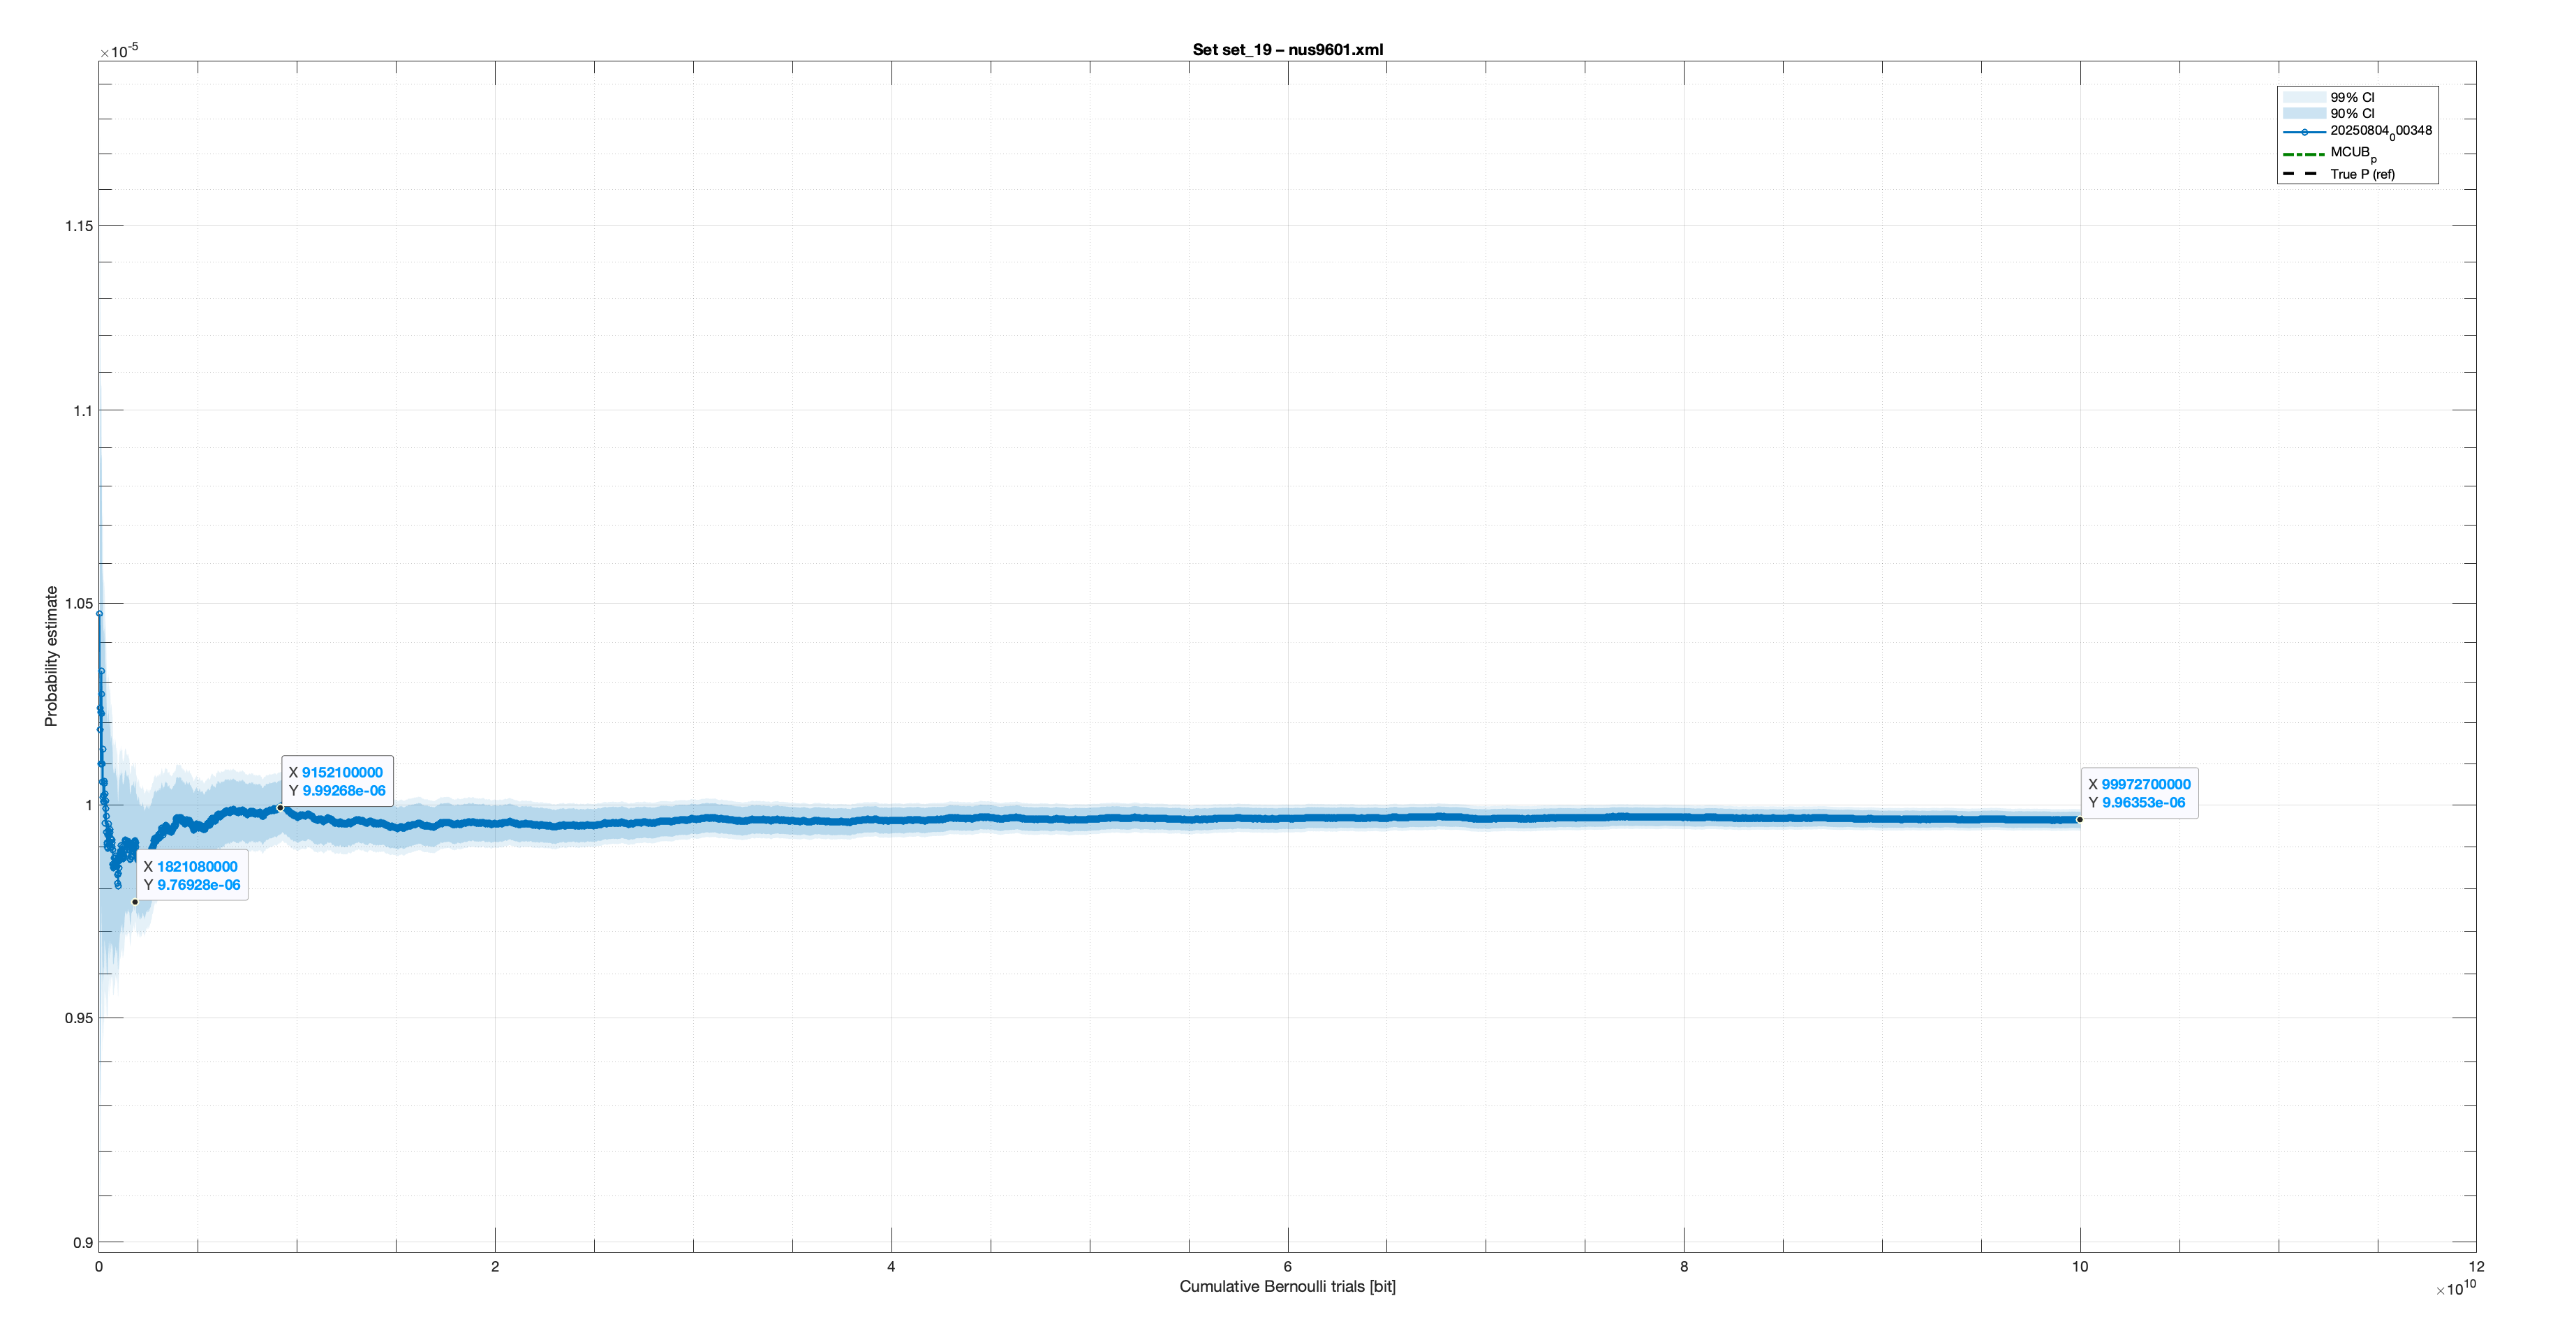
\includegraphics[width=1\textwidth]{4_casestudy/conv_nus9601.eps}
    \label{fig:rare}
\end{figure}
\end{frame}


\subsection{Aralia Fault Tree Data Set - Convergence for Rare Events}
\begin{frame}
    \input{4_casestudy/4_mae}
\end{frame}

% \subsection{Aralia Fault Tree Data Set - Throughput Benchmarks}
% \begin{frame}
%     \begin{figure}[h]
%     \centering
%     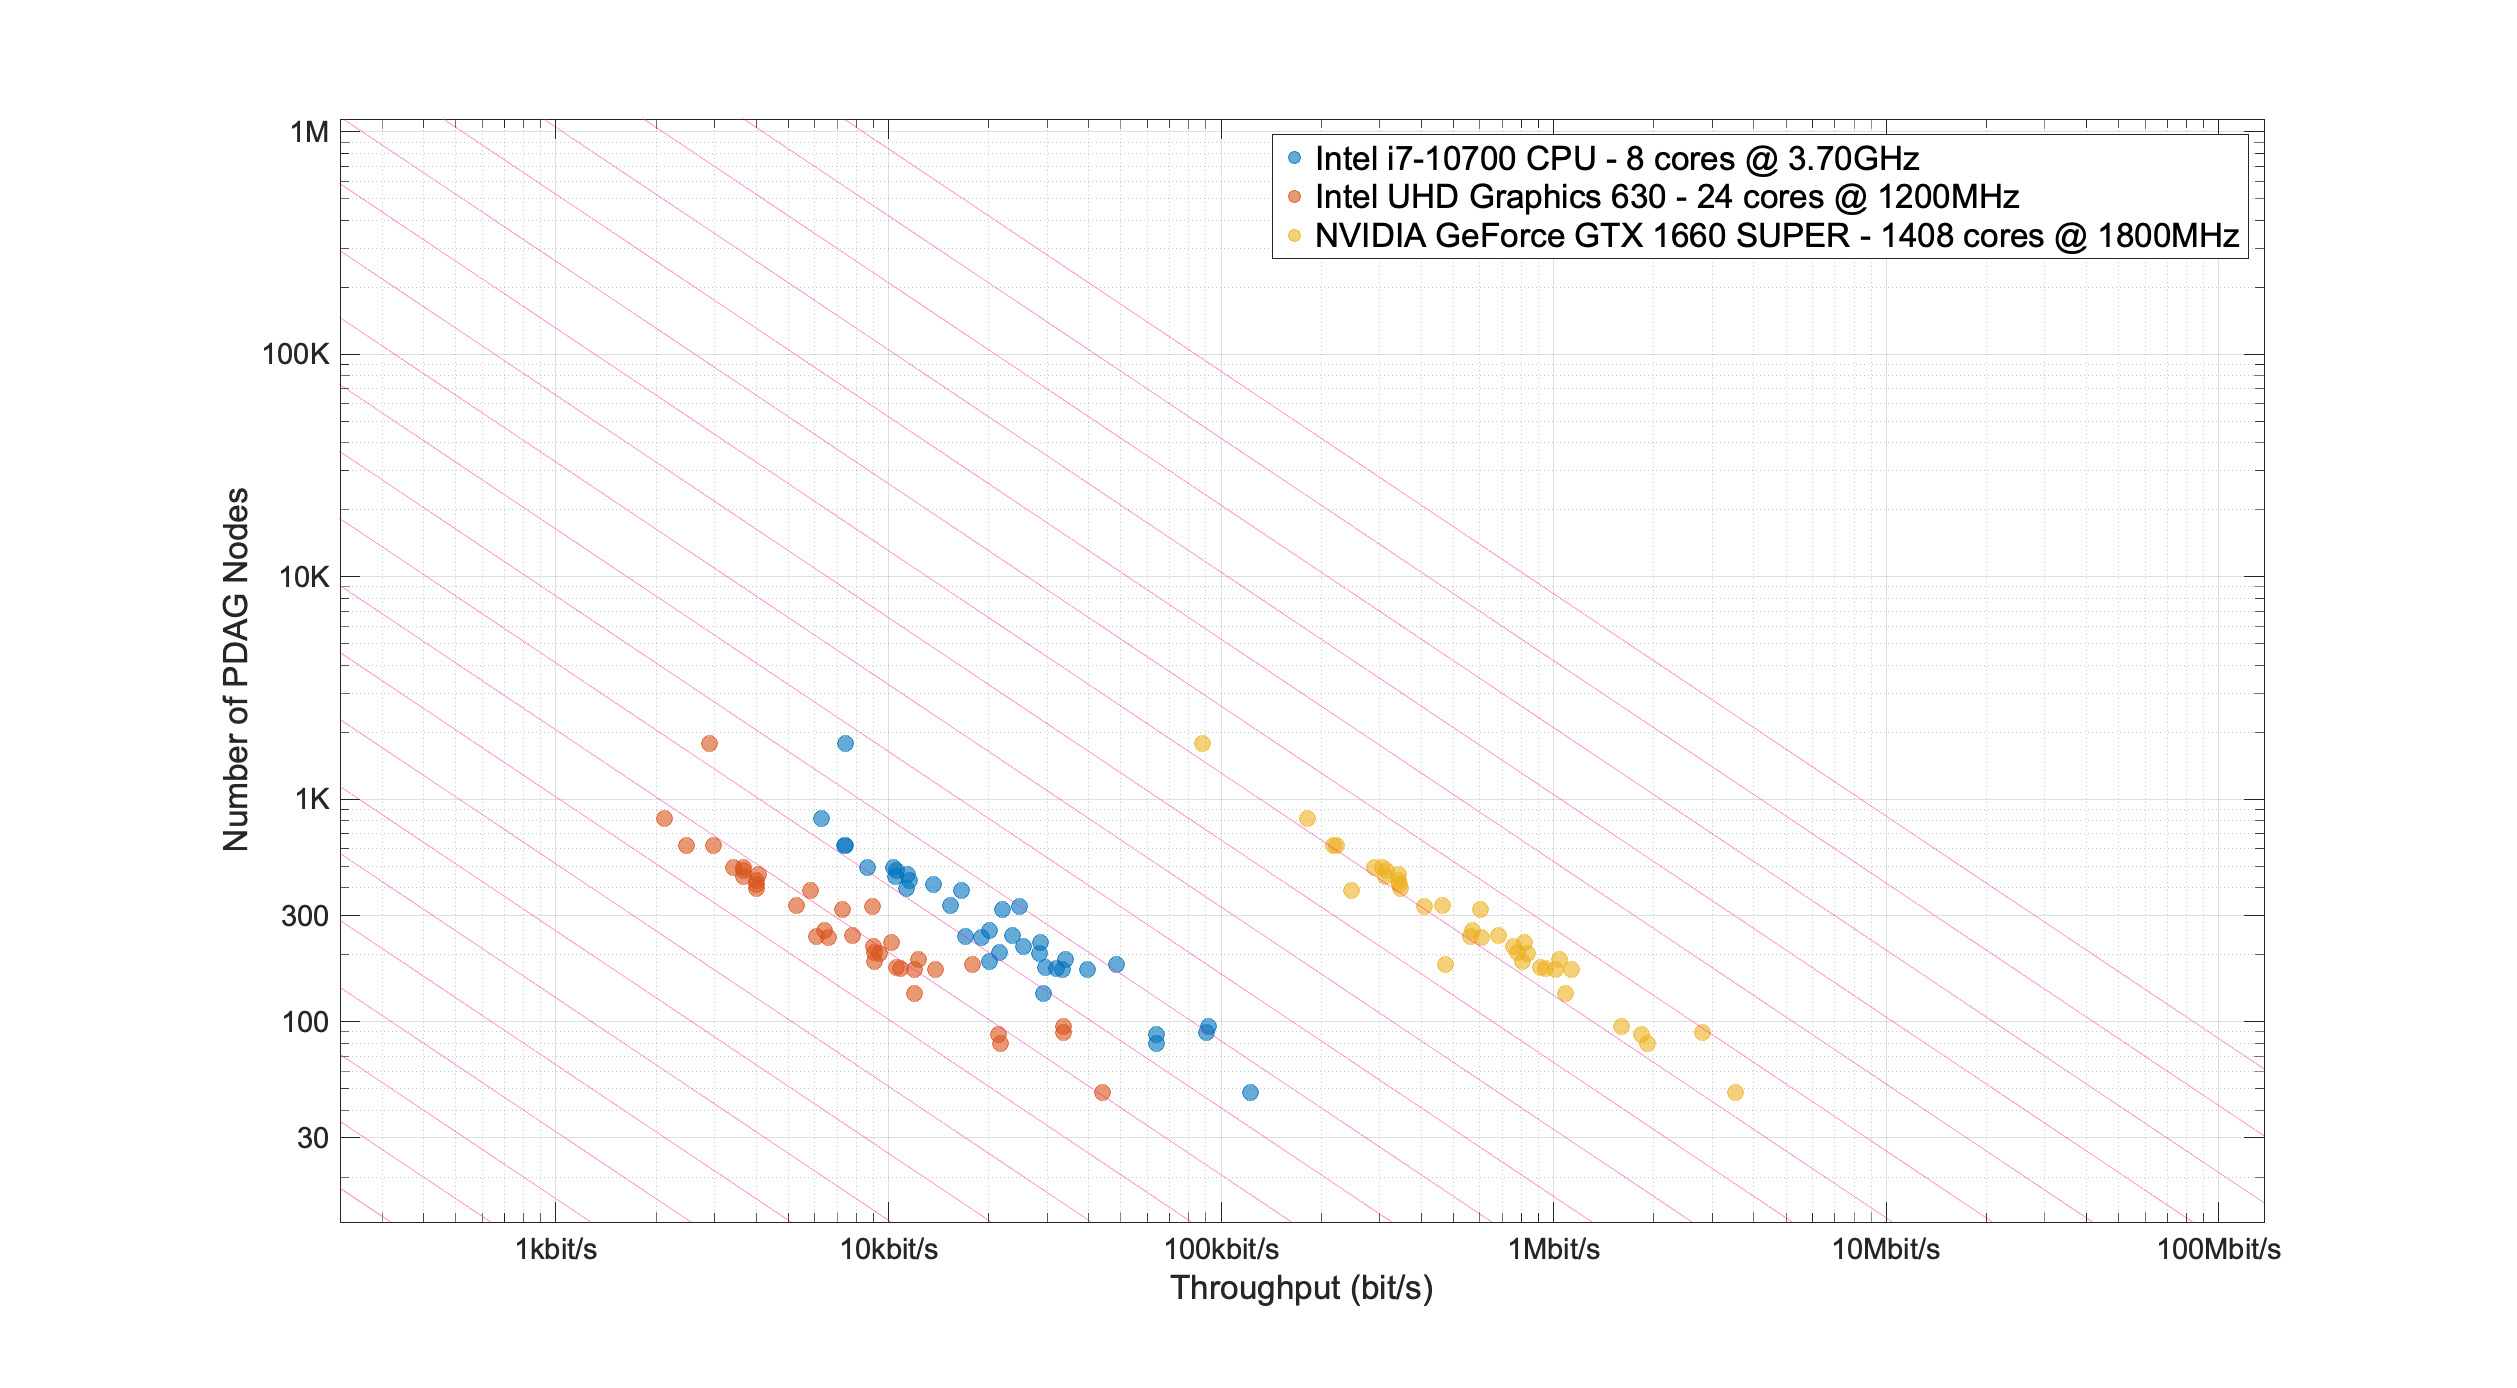
\includegraphics[width=0.9\textwidth]{4_casestudy/throughput/slides_nodes_vs_throughput.eps}
%     \caption{PDAG Node Count vs Throughput [bit/s]}
%     \label{fig:nodes_vs_throughput}
% \end{figure}
% \end{frame}




% \begin{frame}{Aralia Fault Tree Dataset}
% show the input dataset table\\
% \end{frame}

% \subsection{Results}
% \begin{frame}{Mar}
% show the input dataset table\\
% \end{frame}